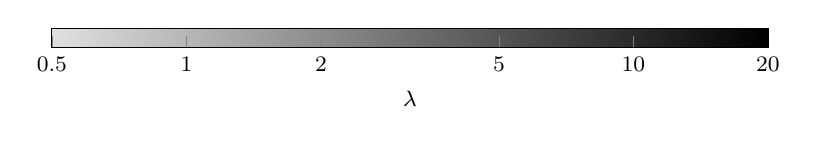
\begin{tikzpicture}
\begin{axis}[
hide axis, scale only axis,
width=0.75\textwidth, height=0pt,
colormap={sigmamap}{rgb(0.0000)=(0.8800,0.8800,0.8800); rgb(0.1000)=(0.7903,0.7903,0.7903); rgb(0.2000)=(0.7040,0.7040,0.7040); rgb(0.3000)=(0.6143,0.6143,0.6143); rgb(0.4000)=(0.5280,0.5280,0.5280); rgb(0.5000)=(0.4383,0.4383,0.4383); rgb(0.6000)=(0.3520,0.3520,0.3520); rgb(0.7000)=(0.2623,0.2623,0.2623); rgb(0.8000)=(0.1760,0.1760,0.1760); rgb(0.9000)=(0.0863,0.0863,0.0863); rgb(1.0000)=(0.0000,0.0000,0.0000)},
point meta min=-0.30103, point meta max=1.30103,
colorbar horizontal,
colorbar style={
  width=0.75\textwidth, height=7pt,
  at={(0,0)}, anchor=north west,
  xlabel={$\lambda$},
  xlabel style={font=\footnotesize},
  tick label style={font=\footnotesize},
  xtick pos=bottom,
  xtick={-0.30103,0,0.30103,0.69897,1,1.30103},
  xticklabels={0.5,1,2,5,10,20},
},
]
\addplot[draw=none] coordinates {(0,0)};
\end{axis}
\end{tikzpicture}
